\section{Result}\label{sec:result}

%--------------------------------------------------------

\subsection{Systematic errors}
\red{TBU} % Error: $|\text{condition\_vary - default}|$ / default * 100 (convert to \%)

\vspace{\columnsep}
\begin{table}[h]
    \centering
    \small
    \begin{tabular}{l|l|l}
    \hline\hline
    Item & Default & Tested \\\hline
    %
    \multicolumn{3}{l}{Online event selection} \\\hline
    ITS-TPC matching & \red{Quote \cite{ana990_Xic0}} & \red{TBU} \\
    Electron track selection & stand (table \ref{tab:eReco}) & vloose, loose, tight, and vtight \\
    \Xis daughter track selection & stand (table \ref{tab:XiReco}) & vloose, loose, tight, and vtight \\
    Rapidity ($|$\textit{y}$|$) interval sensitivity & 0.5 & 0.8 \\\hline
    %
    \multicolumn{3}{l}{Offline event selection} \\\hline
    Electron pID & stand (table \ref{tab:ePID}) & vloose, loose, tight, and vtight \\
    \Xis pID by topology & stand (table \ref{tab:XiPID}) & vloose, loose, tight, and vtight \\
    e-\Xim pair selection: mass & 2.5 (table \ref{tab:eXiPair}) & 2.3 and 2.7 \\
    e-\Xim pair selection: opening angle & 90 (table \ref{tab:eXiPair}) & 70 \\\hline
    %
    \multicolumn{3}{l}{Offline analysis} \\\hline
    Unfolding: method & Bayesian & SVD \\
    Unfolding: \# of iterations & 3 & 2, 4, 5, 6, and 7 \\
    Unfolding: \pt range & [1, 2, 4, 6, 8, 12, 14] & [1, 2, 4, 6, 8, 12] and \\
    && [0, 1, 2, 4, 6, 8, 12, 24] \\
    \Xib over-subtraction correction & \red{Disabled} & \red{TBU} \\
    Feed-down subtraction            & \red{Disabled} & \red{TBU} \\
    Generated \pt shape & Central fit (section \ref{subsubsec:ptWeighting}) & Fit variations \\
    %
    \hline\hline
    \end{tabular}
    \caption{Table of items for systematic error and conditions tested}
    \label{tab:systItems}
\end{table}

\begin{figure}[b]
    \centering
    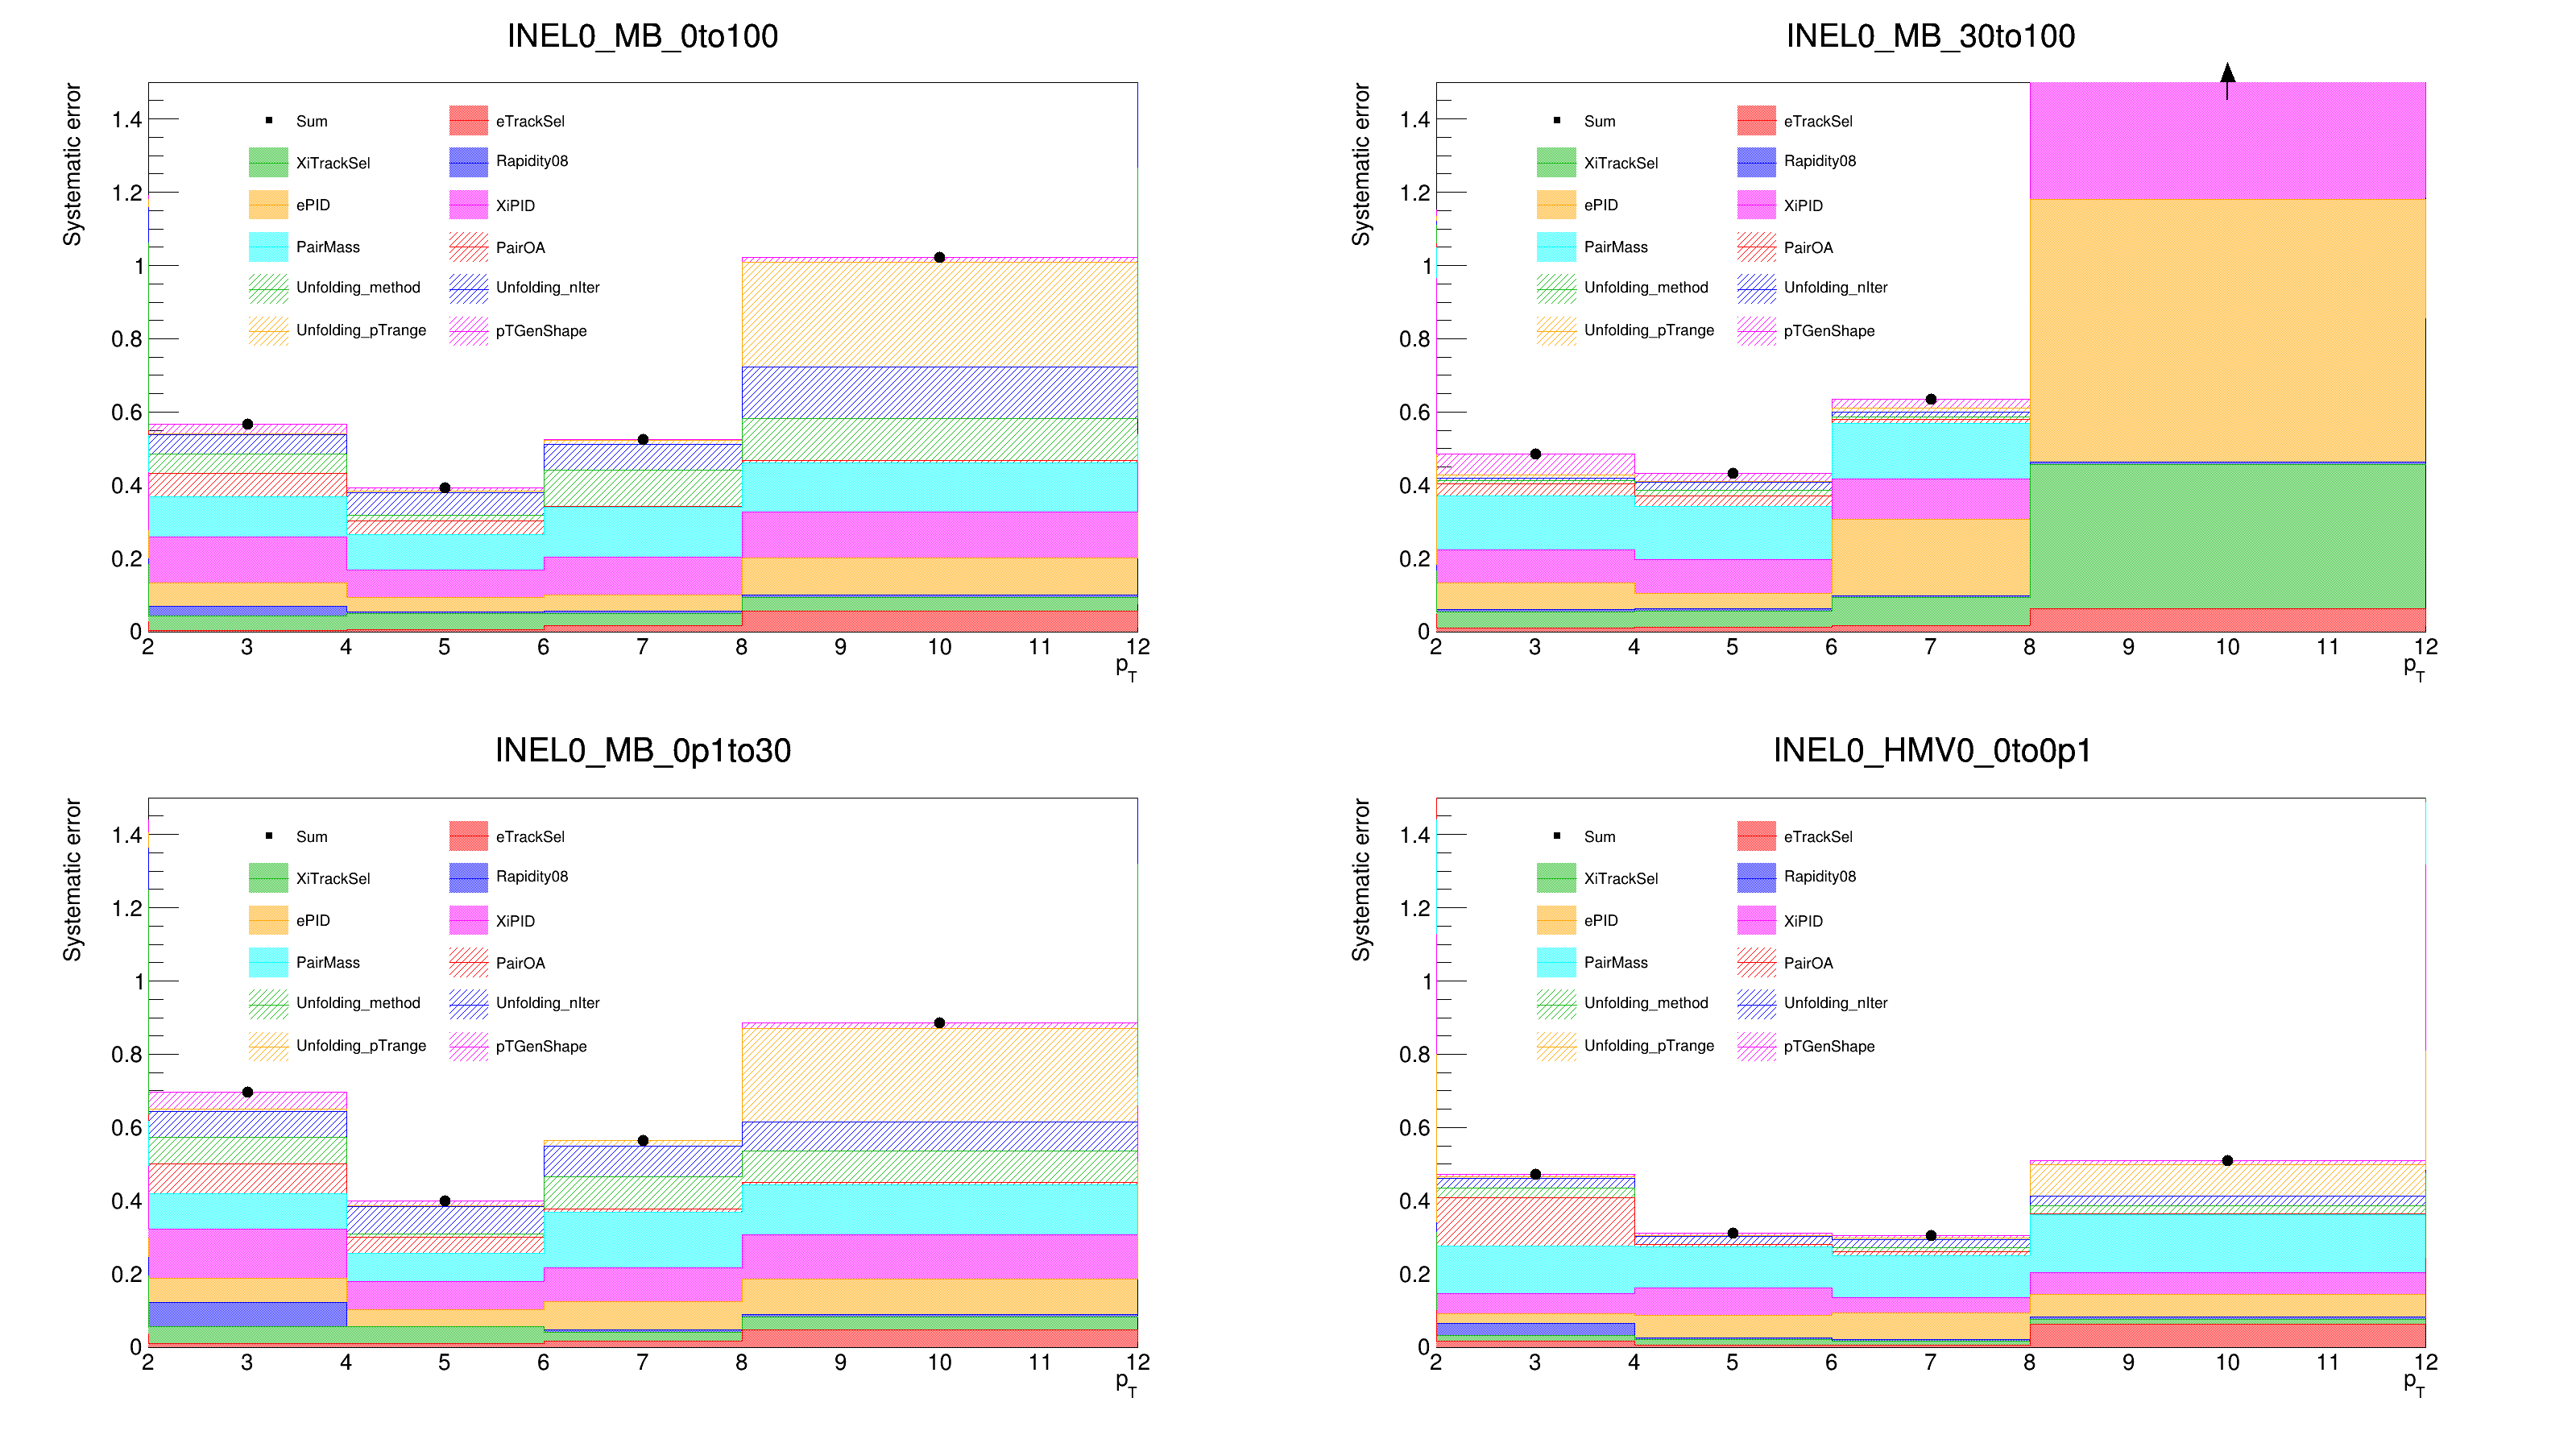
\includegraphics[width=0.925\textwidth]{plots/s3_SystErr_2to12.png}
    \caption{Estimated systematic errors in percentage. Note that the sum is a simple stack of all items.}
    \label{fig:s3_systErr}
\end{figure}

\clearpage
\begin{table}[t]
    \centering
    \small
    \begin{tabular}{l|rrrr}
    \hline\hline
    \multicolumn{5}{c}{\normalsize \blue{MB + [0, 100]}} \\\hline
    \multirow{2}{*}{Item \red{(* error unit: \%)}} & \multicolumn{4}{c}{\pt (\GeVc)} \\\cline{2-5}
    & 2-4 & 4-6 & 6-8 & 8-12 \\\hline
    %
    \multicolumn{5}{l}{Online event selection} \\\hline
    ITS-TPC matching & \red{2.5} & \red{2.5} & \red{2.5} & \red{2.5} \\
    Electron track selection                   &  0.4 &  0.7 &  1.7 &  5.6 \\
    \Xis daughter track selection              &  3.9 &  4.4 &  3.3 &  3.8 \\
    Rapidity (\textit{y}) interval sensitivity &  2.7 &  0.5 &  0.6 &  0.7 \\
    \hline
    %
    \multicolumn{5}{l}{Offline event selection} \\\hline
    Electron pID                         &  6.4 &  3.8 &  4.5 & 10.0 \\
    \Xis pID by topology                 & 12.6 &  7.6 & 10.3 & 12.6 \\
    e-\Xim pair selection: mass          & 10.8 &  9.6 & 13.6 & 13.3 \\
    e-\Xim pair selection: opening angle &  6.4 &  3.7 &  0.3 &  0.7 \\
    \hline
    %
    \multicolumn{5}{l}{Offline analysis} \\\hline
    Unfolding: method                &  5.3 &  1.6 &  9.9 & 11.4 \\
    Unfolding: \# of iterations      &  5.4 &  6.3 &  7.1 & 14.0 \\
    Unfolding: \pt range             &  0.1 &  0.3 &  1.1 & 28.8 \\
    \Xib over-subtraction correction & \multicolumn{4}{c}{\red{TBU}} \\
    Feed-down subtraction            & \multicolumn{4}{c}{\red{TBU}} \\
    Generated \pt shape              &  2.7 &  0.9 &  0.1 &  1.2 \\
    \hline
    %
    Total & 21.2 & 15.7 & 21.9 & 40.6 \\
    \hline\hline
    \end{tabular}
    \caption{Table of systematic errors for configuration MB + [0, 100]}
    \label{tab:systMB_0to100}
\end{table}

\begin{table}[b]
    \centering
    \small
    \begin{tabular}{l|rrrr}
    \hline\hline
    \multicolumn{5}{c}{\normalsize \blue{MB + [30, 100]}} \\\hline
    \multirow{2}{*}{Item \red{(* error unit: \%)}} & \multicolumn{4}{c}{\pt (\GeVc)} \\\cline{2-5}
    & 2-4 & 4-6 & 6-8 & 8-12 \\\hline
    %
    \multicolumn{5}{l}{Online event selection} \\\hline
    ITS-TPC matching & \red{2.5} & \red{2.5} & \red{2.5} & \red{2.5} \\
    Electron track selection                   &  1.1 &  1.3 &  1.7 &  6.4 \\
    \Xis daughter track selection              &  4.2 &  4.4 &  7.6 & 39.3 \\
    Rapidity (\textit{y}) interval sensitivity &  0.7 &  0.8 &  0.5 &  0.7 \\
    \hline
    %
    \multicolumn{5}{l}{Offline event selection} \\\hline
    Electron pID                         &  7.3 &  4.0 & 21.0 & 71.7 \\
    \Xis pID by topology                 &  9.2 &  9.4 & 10.9 & 79.1 \\
    e-\Xim pair selection: mass          & 14.5 & 14.3 & 15.1 & 22.7 \\
    e-\Xim pair selection: opening angle &  3.3 &  3.0 &  1.1 &  0.9 \\
    \hline
    %
    \multicolumn{5}{l}{Offline analysis} \\\hline
    Unfolding: method                &  0.9 &  1.4 &  0.8 & 89.3 \\
    Unfolding: \# of iterations      &  0.8 &  2.3 &  1.2 & 60.2 \\
    Unfolding: \pt range             &  0.8 &  0.2 &  1.1 & 32.5 \\
    \Xib over-subtraction correction & \multicolumn{4}{c}{\red{TBU}} \\
    Feed-down subtraction            & \multicolumn{4}{c}{\red{TBU}} \\
    Generated \pt shape              &  5.7 &  2.1 &  2.3 &  0.8 \\
    \hline
    %
    Total & 20.5 & 18.9 & 29.4 & 161.8 \\
    \hline\hline
    \end{tabular}
    \caption{Table of systematic errors for configuration MB + [30, 100]}
    \label{tab:systMB_30to100}
\end{table}

\clearpage
\begin{table}[t]
    \centering
    \small
    \begin{tabular}{l|rrrrr}
    \hline\hline
    \multicolumn{5}{c}{\normalsize \blue{MB + [0.1, 30]}} \\\hline
    \multirow{2}{*}{Item \red{(* error unit: \%)}} & \multicolumn{4}{c}{\pt (\GeVc)} \\\cline{2-5}
    & 2-4 & 4-6 & 6-8 & 8-12 \\\hline
    %
    \multicolumn{5}{l}{Online event selection} \\\hline
    ITS-TPC matching & \red{2.5} & \red{2.5} & \red{2.5} & \red{2.5} \\
    Electron track selection                   &  1.1 &  1.0 &  1.8 &  4.7 \\
    \Xis daughter track selection              &  4.5 &  4.6 &  2.4 &  3.5 \\
    Rapidity (\textit{y}) interval sensitivity &  6.6 &  0.0 &  0.6 &  0.7 \\
    \hline
    %
    \multicolumn{5}{l}{Offline event selection} \\\hline
    Electron pID                         &  6.6 &  4.5 &  7.6 &  9.8 \\
    \Xis pID by topology                 & 13.6 &  7.7 &  9.3 & 12.1 \\
    e-\Xim pair selection: mass          &  9.5 &  7.9 & 15.2 & 13.5 \\
    e-\Xim pair selection: opening angle &  8.3 &  4.3 &  0.8 &  0.8 \\
    \hline
    %
    \multicolumn{5}{l}{Offline analysis} \\\hline
    Unfolding: method                &  7.3 &  0.8 &  8.9 &  8.6 \\
    Unfolding: \# of iterations      &  7.1 &  7.5 &  8.3 &  7.9 \\
    Unfolding: \pt range             &  0.5 &  0.3 &  1.4 & 25.3 \\
    \Xib over-subtraction correction & \multicolumn{4}{c}{\red{TBU}} \\
    Feed-down subtraction            & \multicolumn{4}{c}{\red{TBU}} \\
    Generated \pt shape              &  4.8 &  1.1 &  0.1 &  1.6 \\
    \hline
    %
    Total & 24.1 & 15.7 & 23.3 & 35.3 \\
    \hline\hline
    \end{tabular}
    \caption{Table of systematic errors for configuration MB + [0.1, 30]}
    \label{tab:systMB_0p1to30}
\end{table}

\begin{table}[b]
    \centering
    \small
    \begin{tabular}{l|rrrrr}
    \hline\hline
    \multicolumn{5}{c}{\normalsize \blue{HMV0 + [0, 0.1]}} \\\hline
    \multirow{2}{*}{Item \red{(* error unit: \%)}} & \multicolumn{4}{c}{\pt (\GeVc)} \\\cline{2-5}
    & 2-4 & 4-6 & 6-8 & 8-12 \\\hline
    %
    \multicolumn{5}{l}{Online event selection} \\\hline
    ITS-TPC matching & \red{2.5} & \red{2.5} & \red{2.5} & \red{2.5} \\
    Electron track selection                   &  1.7 &  0.6 &  0.6 &  6.4 \\
    \Xis daughter track selection              &  1.5 &  1.6 &  1.1 &  1.3 \\
    Rapidity (\textit{y}) interval sensitivity &  3.4 &  0.3 &  0.5 &  0.7 \\
    \hline
    %
    \multicolumn{5}{l}{Offline event selection} \\\hline
    Electron pID                         &  2.6 &  6.2 &  7.2 &  6.1 \\
    \Xis pID by topology                 &  5.5 &  7.4 &  4.1 &  5.9 \\
    e-\Xim pair selection: mass          & 12.9 & 11.3 & 11.6 & 15.8 \\
    e-\Xim pair selection: opening angle & 13.3 &  0.6 &  0.9 &  0.3 \\
    \hline
    %
    \multicolumn{5}{l}{Offline analysis} \\\hline
    Unfolding: method                &  2.5 &  0.0 &  1.1 &  2.2 \\
    Unfolding: \# of iterations      &  2.7 &  2.3 &  2.2 &  2.7 \\
    Unfolding: \pt range             &  0.4 &  0.1 &  0.6 &  8.5 \\
    \Xib over-subtraction correction & \multicolumn{4}{c}{\red{TBU}} \\
    Feed-down subtraction            & \multicolumn{4}{c}{\red{TBU}} \\
    Generated \pt shape              &  0.8 &  0.6 &  0.5 &  1.1 \\
    \hline
    %
    Total & 20.4 & 15.4 & 14.8 & 21.4 \\
    \hline\hline
    \end{tabular}
    \caption{Table of systematic errors for configuration HMV0 + [0, 0.1]}
    \label{tab:systHMV0_0to0p1}
\end{table}

\iffalse
\begin{table}[h]
    \centering
    \small
    \begin{tabular}{l|r|r|r|r|r|r}
    \hline\hline
    \multicolumn{7}{c}{\normalsize \blue{CONF}} \\\hline
    \multirow{2}{*}{Item} & \multicolumn{6}{c}{\pt (\GeVc)} \\\cline{2-7}
    & 1-2 & 2-4 & 4-6 & 6-8 & 8-12 & 12-24 \\\hline
    %
    \multicolumn{7}{l}{Online event selection} \\\hline
    ITS-TPC matching                           & & & \red{2.5} & & & \\
    Electron track selection                   & & & & & & \\
    \Xis daughter track selection              & & & & & & \\
    Rapidity (\textit{y}) interval sensitivity & & & & & & \\
    \hline
    %
    \multicolumn{7}{l}{Offline event selection} \\\hline
    Electron pID                         & & & & & & \\
    \Xis pID by topology                 & & & & & & \\
    e-\Xim pair selection: mass          & & & & & & \\
    e-\Xim pair selection: opening angle & & & & & & \\\hline
    %
    \multicolumn{7}{l}{Offline analysis} \\\hline
    Unfolding: method                & & & & & & \\
    Unfolding: \# of iterations      & & & & & & \\
    Unfolding: \pt range and binning & & & & & & \\
    \Xib over-subtraction correction & & & & & & \\
    Feed-down subtraction            & & & & & & \\
    Generated \pt shape              & & & & & & \\\hline
    %
    Total & & & & & & \\
    %
    \hline\hline
    \end{tabular}
    \caption{Table of systematic errors]}
    \label{tab:syst}
\end{table}
\fi

\clearpage
%--------------------------------------------------------

\subsection{\Xic yields and \Xic/\Dzero ratio}
\red{TBU}

\begin{figure}[h]
    \centering
    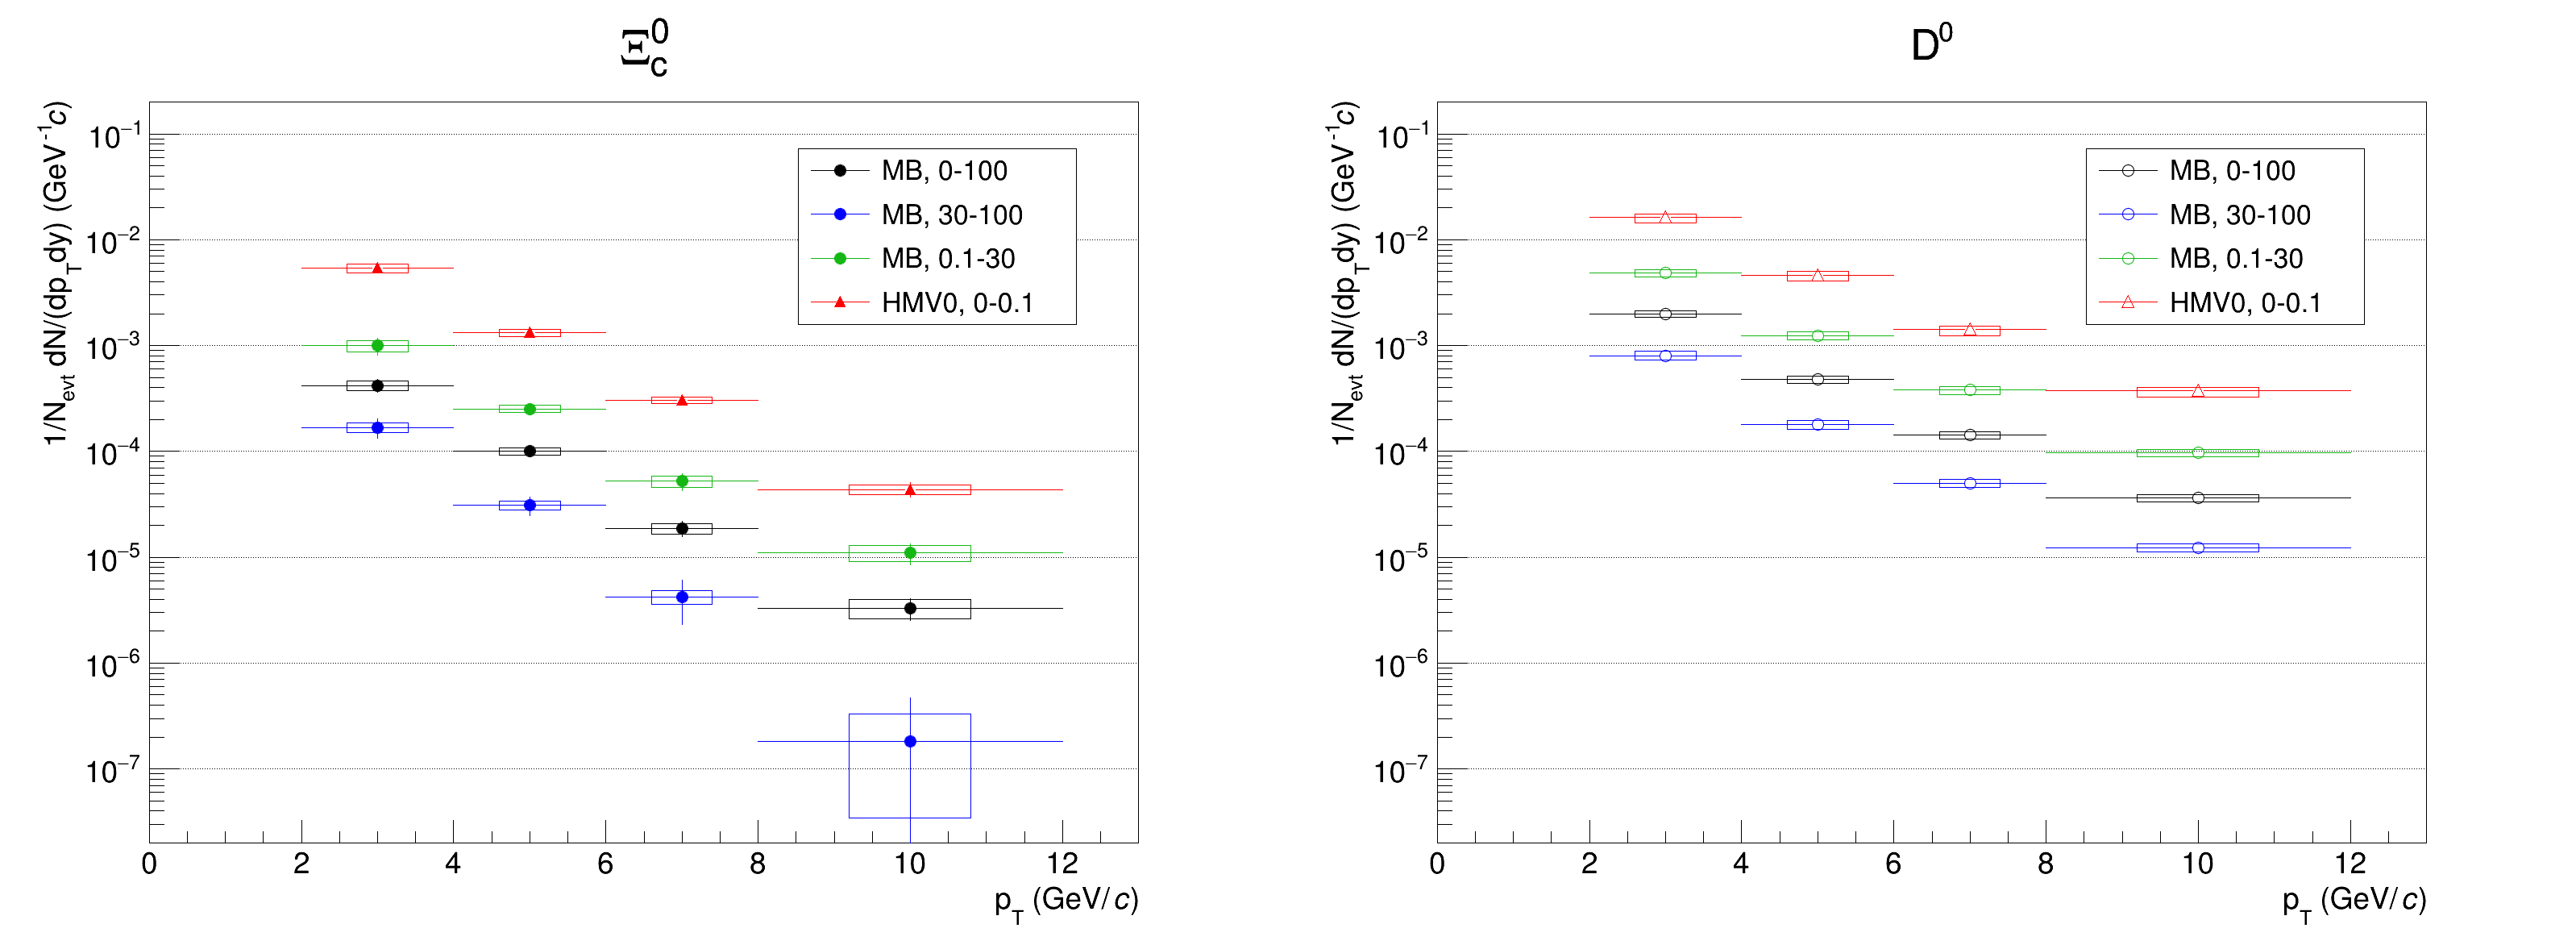
\includegraphics[width=0.95\textwidth]{plots/s3_Yield_INEL0.png}
    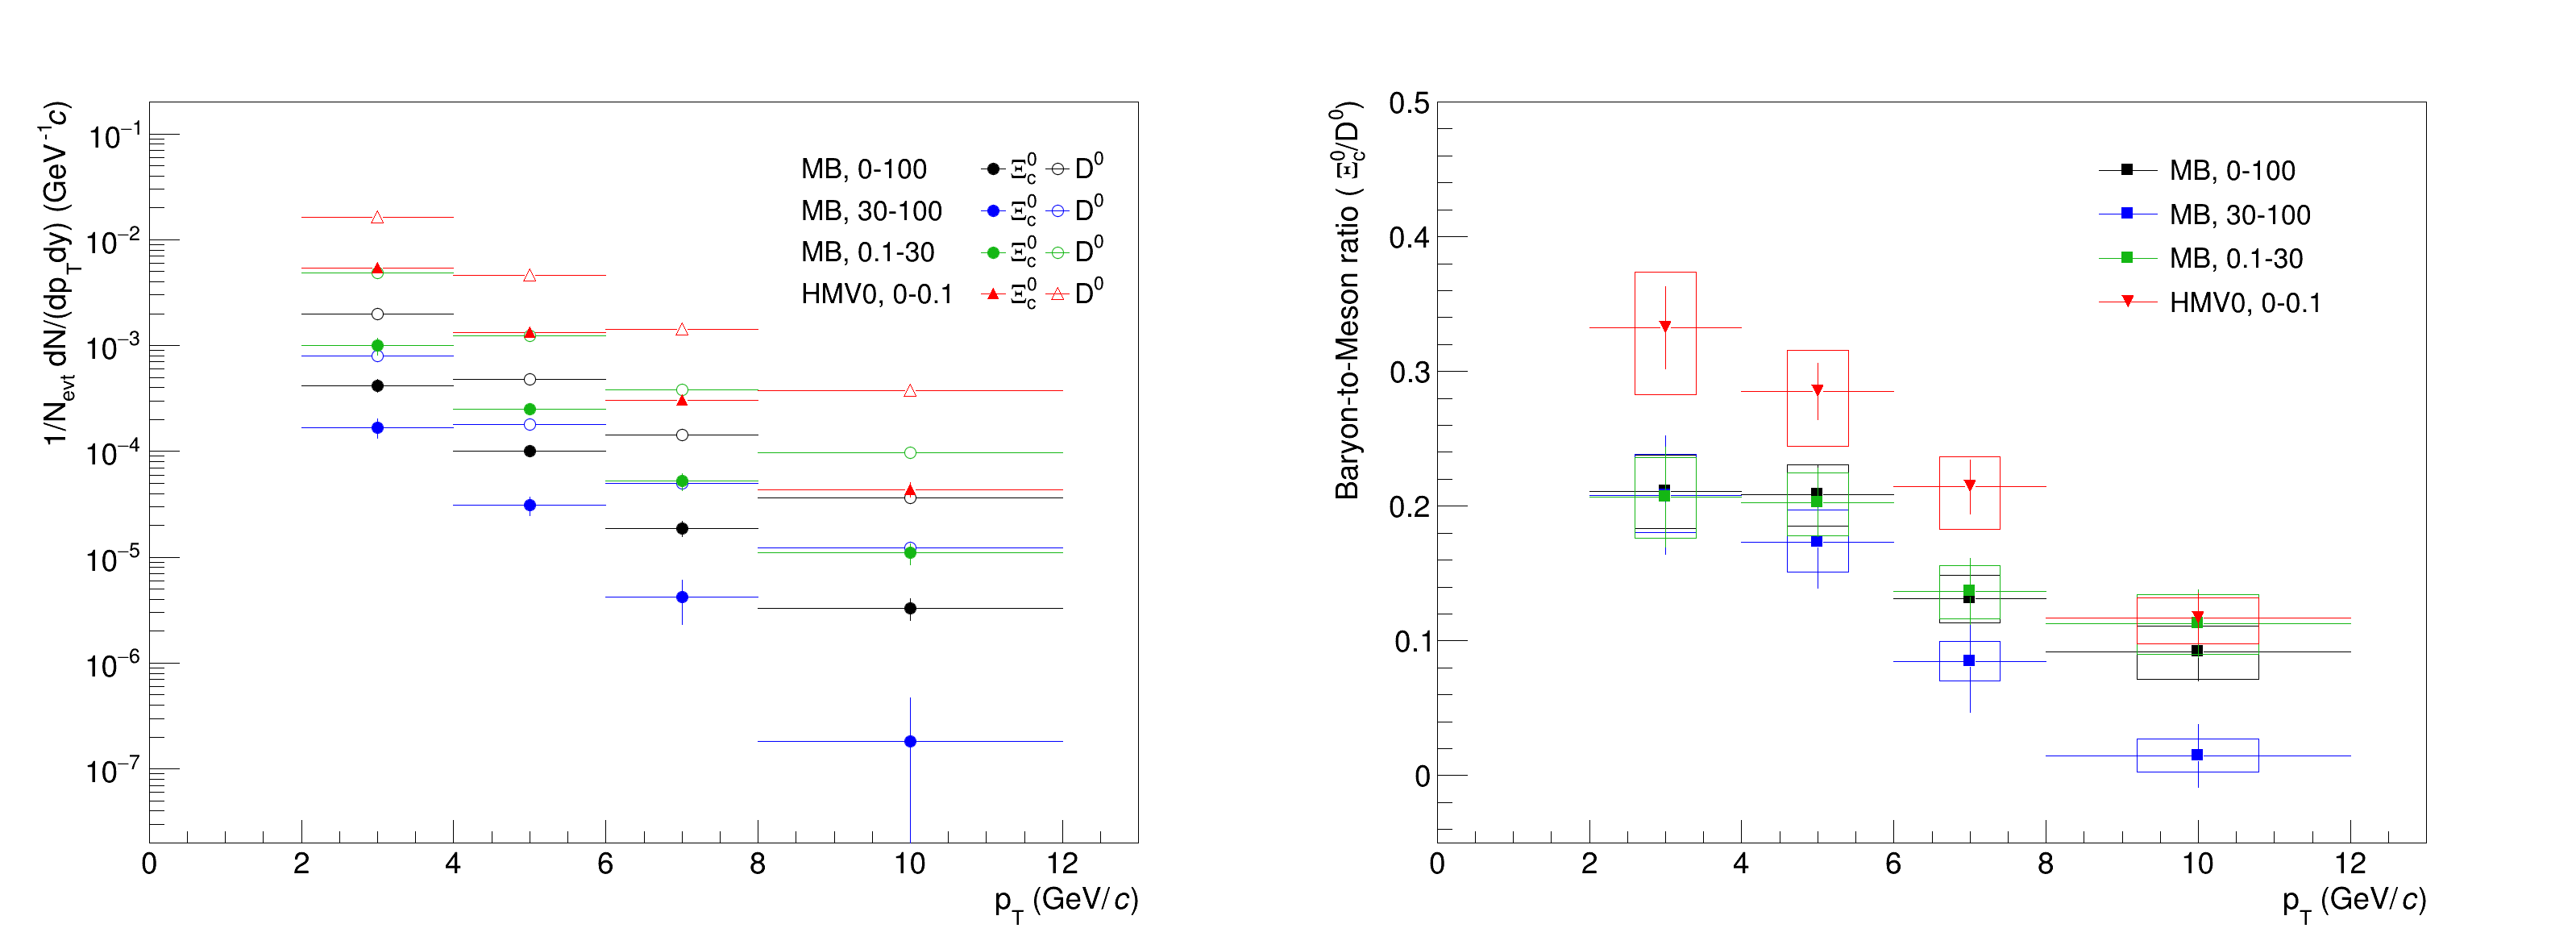
\includegraphics[width=0.95\textwidth]{plots/s3_Ratio_INEL0.png}
    \caption{Normalized invariant cross-section of \Xic (top left) and \Dzero (top right) \cite{ana993_D0}.
    The bottom left shows the cross-sections together and The bottom right shows the baryon-to-meson ratio calculated by \Xic/\Dzero.}
    \label{fig:s3_results}
\end{figure}

